\documentclass[11pt,a4paper]{article}
\usepackage[utf8]{inputenc}
\DeclareUnicodeCharacter{00A0}{ } % because overleaf can be weird (and smuggle in no-break-spaces(?))
\usepackage[english]{babel}
\usepackage{amsmath}
\usepackage{amsfonts}
\usepackage{amssymb}
\usepackage{makeidx}
\usepackage{graphicx}
\usepackage{subcaption} % also for subfigure
\usepackage{fourier}
\usepackage[left=2cm,right=2cm,top=2cm,bottom=2cm]{geometry}
\usepackage[style=english]{csquotes}

\usepackage{amsthm} % for proofs
\usepackage{mathtools} % for \xRightarrow{Text über Implikationspfeil}
\usepackage[mathcal]{euscript} % e.g. use \mathcal{A} for script A
\usepackage{todonotes}
\usepackage{IEEEtrantools} % for IEEEeqnarray, see https://moser-isi.ethz.ch/docs/typeset_equations.pdf for details
\usepackage{textcomp} % for copyright symbols
\usepackage{marvosym} % for \Corresponds symbol


\author{Florian Anke, Alexander Niggemeier, Dennis Sehring, Lukas Stratmann}
\title{Spaceship Documentation}

\usepackage[hidelinks,
	pdfauthor={Florian Anke, Alexander Niggemeier, Dennis Sehring, Lukas Stratmann},
	pdftitle={Spaceship -- Documentation},
	pdfproducer={LaTeX with hyperref},
	pdfcreator={pdflatex}]{hyperref}


\setlength{\parindent}{0pt}
\setlength{\parskip}{6pt}

\emergencystretch=1em % prevents some overfull \hbox warnings

%\usepackage[style=ieee,backend=biber]{biblatex} % APA style as demanded in "Leitfaden Wissenschaftliches Arbeiten KS.pdf", requires texlive-bibtex-extra
%\DeclareLanguageMapping{german}{german-apa}
%\addbibresource{literature.bib} % run compile_bibliography.sh first, requires biber



\begin{document}
	\begin{titlepage}
		\begin{center}
			
\includegraphics[width=.7\textwidth]{Logo_Uni_Paderborn}
			
			\vspace{2cm}			
			
			\LARGE{\textbf{Spaceship}} \\
            \vspace{.3cm}
            \Large{\textbf{Proseminar Games Engineering}} \\
			\vspace{.7cm}
			\LARGE{Documentation} \\
			
			\vspace{4cm}
			
			\Large{\textbf{Authors}} \\
			\medskip
			
			\begin{tabular}{|l|l|l|} \hline
            	Florian Anke		& \texttt{6691498}			& \href{mailto:fanke@mail.upb.de}{fanke@mail.upb.de} \\ \hline
                Alexander Niggemeier	& \texttt{6681367}		& \href{mailto:aniggem1@mail.upb.de}{aniggem1@mail.upb.de} \\ \hline
				Dennis Sehring		& \texttt{7002663} 	& \href{mailto:dsehring@mail.upb.de}{dsehring@mail.upb.de} \\ \hline
				Lukas Stratmann		& \texttt{7005026} 	& \href{mailto:lumpiluk@mail.upb.de}{lumpiluk@mail.upb.de} \\ \hline
			\end{tabular}
		\end{center}
	\end{titlepage}
	
	\newpage
	
    \tableofcontents
    \newpage
    
    \section{The Game}
    
    	\subsection{Installation}
        
        	\subsubsection{End Users}
            	
                Download from Sciebo (includes project files and executables)\\
                \href{https://uni-paderborn.sciebo.de/index.php/s/E9BuBwsgwINEkTU}{https://uni-paderborn.sciebo.de/index.php/s/E9BuBwsgwINEkTU} \\
                Password: Games
        
        	\subsubsection{Developers}
            
                Clone the project from: \\
                irb-git@git.cs.upb.de:dsehring/team-spaceship.git (\href{https://git.cs.upb.de/dsehring/team-spaceship}{https://git.cs.upb.de/dsehring/team-spaceship})\\
                Or download it from sciebo like end users and take the project folder.
                
                Then launch the \enquote{Spaceship.uproject} file.
        
        \subsection{Controls}
        	
            \begin{tabular}{ll}
            	Mouse movement: & Control ship \\
                Left mouse button (LMB): & Shoot laser (only near asteroid fields) \\
                Right mouse button (RMB): & Use turbo \\
                ESC: & Open pause menu \\
            \end{tabular}
            
        \subsection{Tutorial}
        
        	After starting the game you are given an interactive tutorial which explains the goal and the controls of this game.
The real game begins when you successfully completed the tutorial.
    
    	\subsection{Mission}
        
        	You are taking part in a race in low earth orbit. In your path are layed out an array of space stations with the potential to charge your turbo reserves. Occasionally, you will also encounter small asteroid fields, which are usually artifacts of sloppy asteroid mining. These asteroids you should avoid, since they will slow you down if you hit them.
        
        	Use the mouse to control your ship and fly through the correct ring of each space station. When approaching a space station, the four lights in two pairs will flash in short intervals. Fly through the ring between the first light of the first pair, and the first light of the second pair.
        
        	You can acquire turbo by flying through space station rings. Depending on how well you are discerning the flashing lights by flying through rings accordingly, you will receive more turbo and hence will be able to finish the race earlier. Your current amount available is displayed at the bottom of the screen. Press and hold RMB to use turbo and boost your ship's speed.
            
        \subsection{Motivation}
        
        	The core motivator of our game is it's racing aspect. We assume that a player wants to finish early in order to get placed high on the highscore list. To not lose speed, the player must avoid colliding with space stations and asteroids. Of course, once she has reached maximum speed, the player could hypothetically keep steering to the sides and avoid the space stations altogether. In order to make this scenario less desireable, the maximum speed that can be reached using turbo is somewhat higher than the regular maximum speed. Furthermore, the player will decelerate back to regular speed once turbo has been deactivated.
            
            
            
    \section{The Experiment}
    
    	The purpose of this project is to see how well certain perception experiments may be embedded in games and, in turn, how much these games can help to make long experiments less tiresome. The experiment we use for this purpose examines the following hypothesis: Higher-brightness stimuli contrasted against surrounding lower-brightness background stimuli are more salient and will be perceived earlier than said background stimuli.
        
        A space station (cf. \autoref{img:spacestationindices}) consists of four rings and four lights. Two lights in opposing corners form one pair. On each encounter with a space station the player will make two temporal order judgments (TOJs) by opting for a ring to fly through. Presently, only one of these TOJs will include the brighter target stimulus.
        
        \begin{figure}[h!tbp]
            \centering
            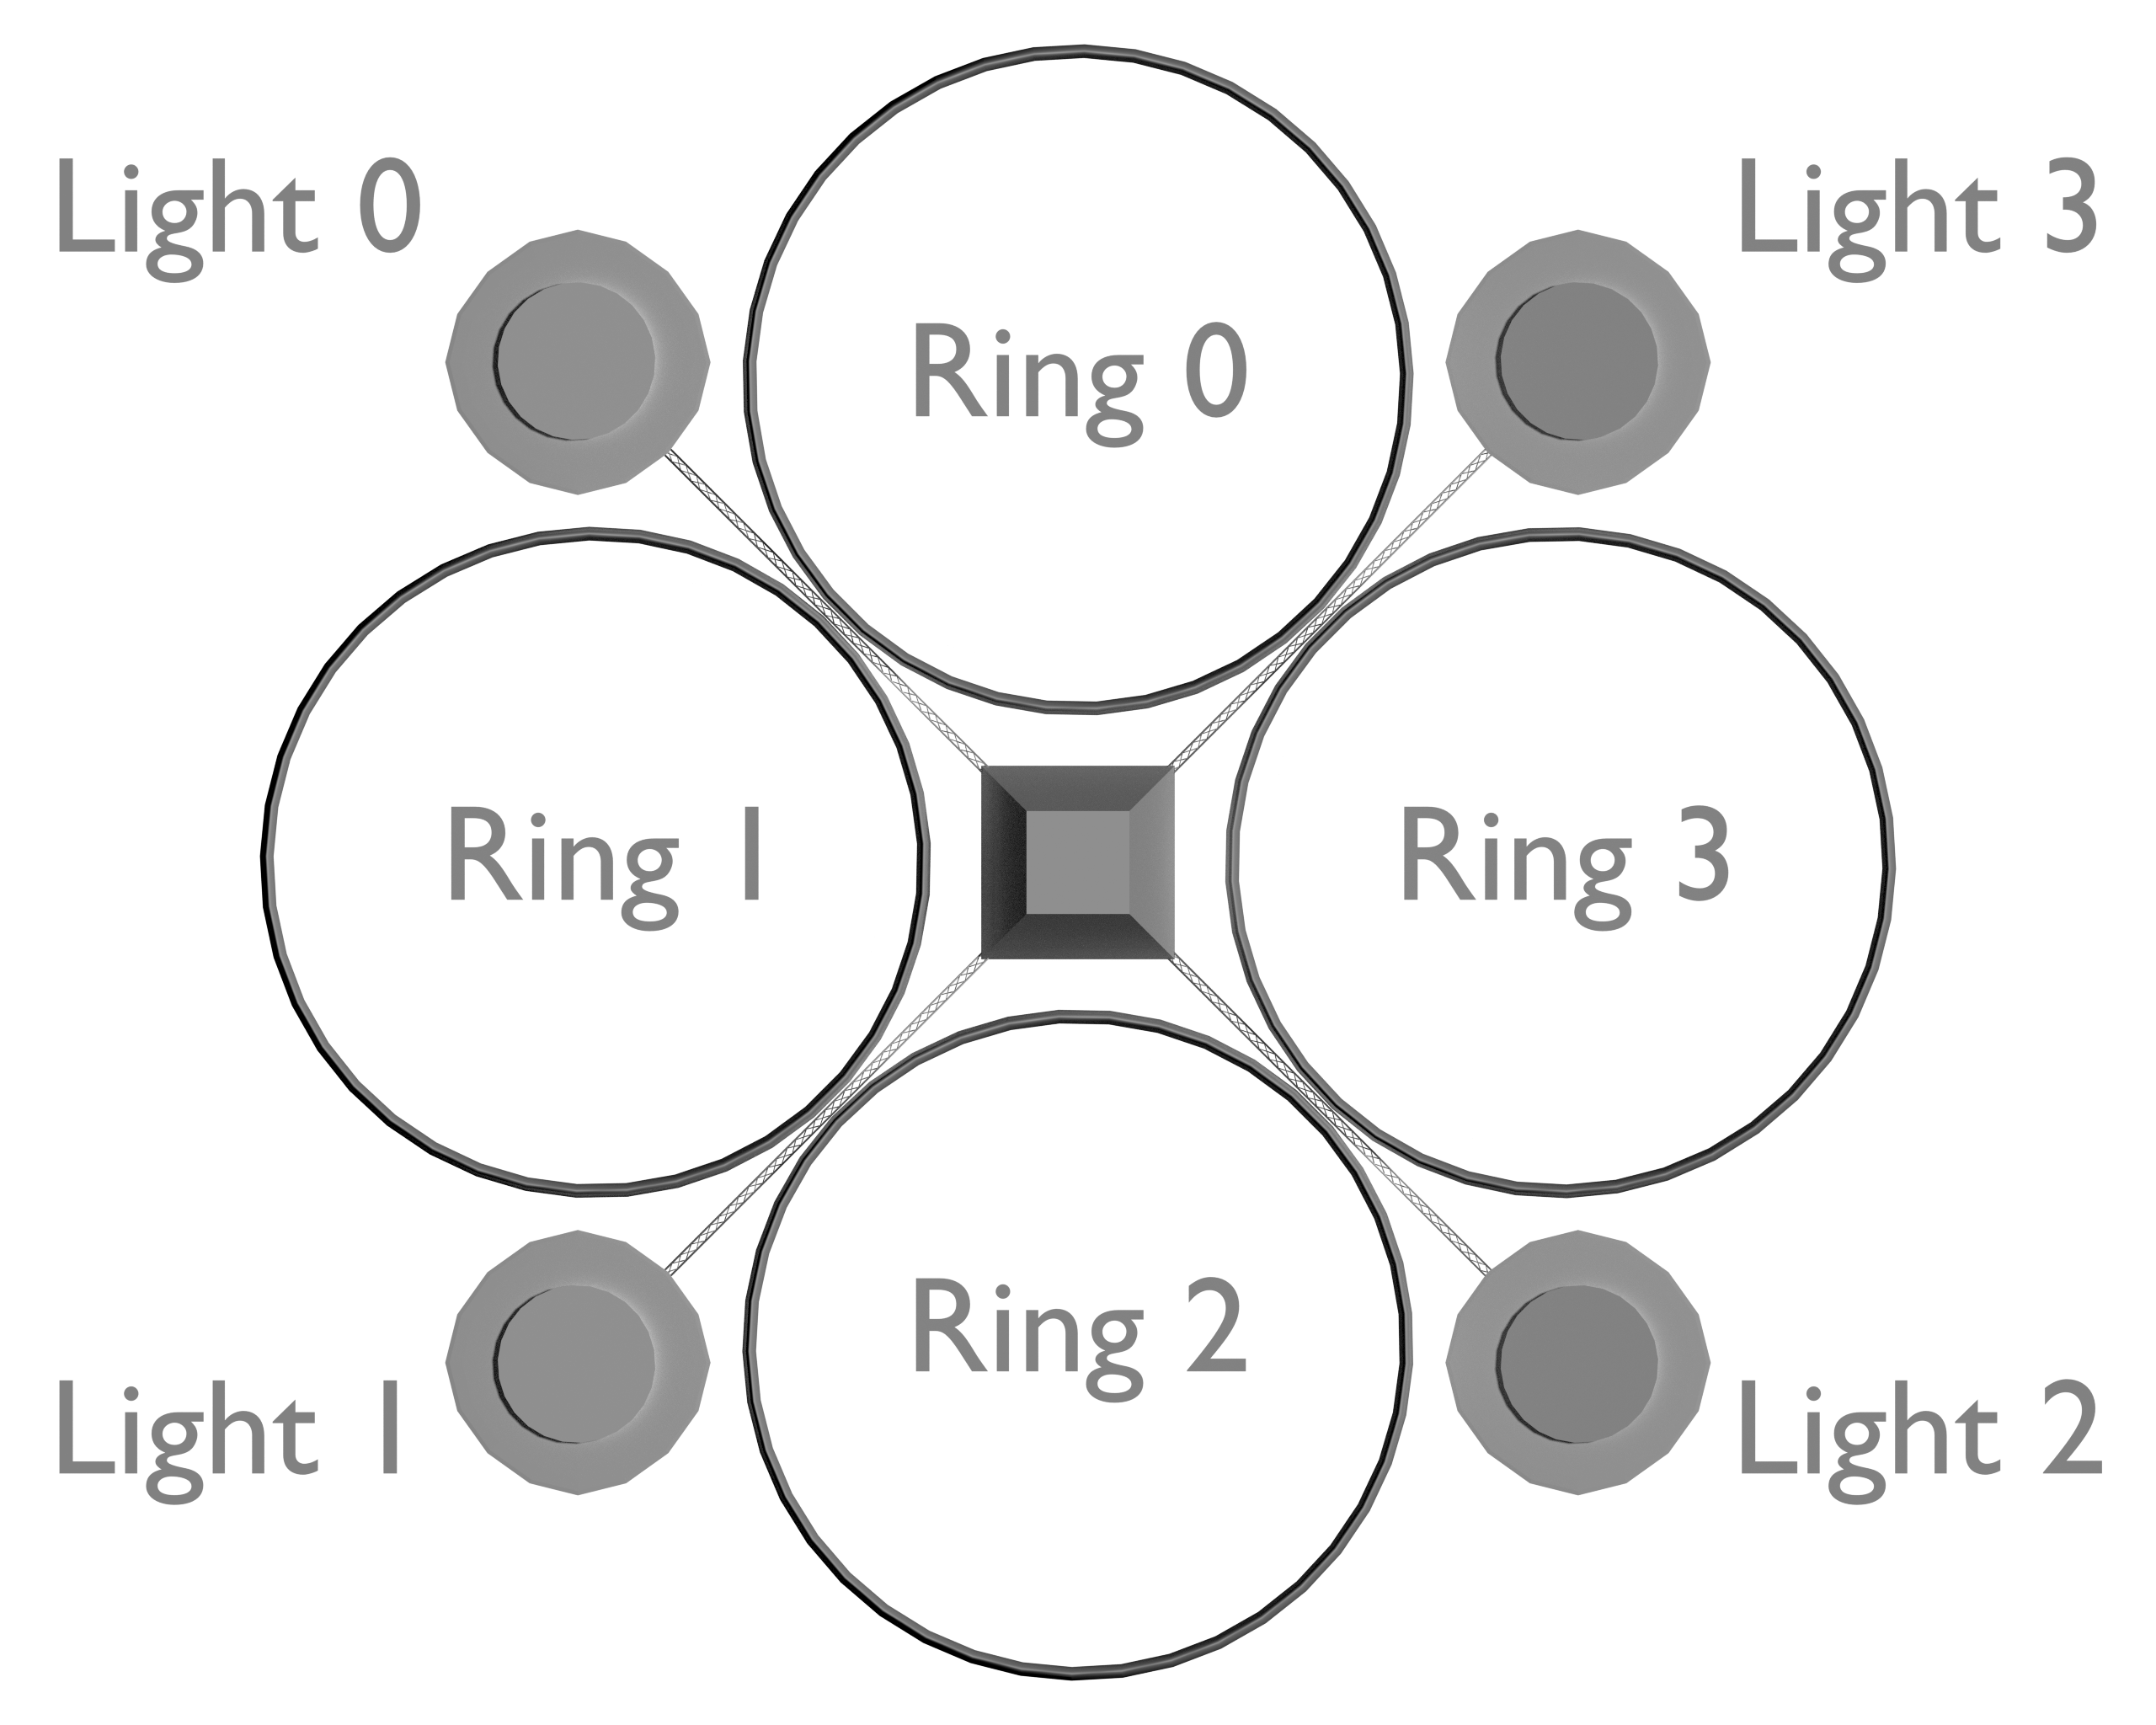
\includegraphics[width=.7\textwidth]{img/spacestation_indices}
            \caption{A space station with light and ring indices.}
            \label{img:spacestationindices}
        \end{figure}
        
        \subsection{Independent Variables}
        
        	We used the following stimulus onset asynchronies (SOAs) in our experiment. However, these can be easily changed if so desired (cf. \autoref{sec:blueprints}).
            \begin{table}[h!tbp]
            	\centering
           		\begin{tabular}{|l|l|l|l|l|} \hline
            		-100ms & -50ms & 0ms & 50ms & 100ms \\ \hline
            	\end{tabular}
                \caption{SOAs used in the experiment.}
                \label{tab:soas}
            \end{table}
            
            Our target luminances can be found in \autoref{tab:lum}. The three background stimuli always used the lowest value. By default, the player will encounter 700 space stations in addition to those spawned during the tutorial, resulting in 700 usable trials. In our test runs we managed to finish the game after about 45 minutes.
            
            \begin{table}[h!tbp]
            	\centering
                \begin{tabular}{|l|l|l|l|} \hline
                	0.345 & 0.471 & 0.596 & 0.878 \\ \hline
                \end{tabular}
                \caption{Luminance values used in the experiment.}
                \label{tab:lum}
            \end{table}  
        
    
    \section{Technical Aspects}
    
        \subsection{Required Software for Development}
    
    	    \begin{itemize}
        	    \item Unreal Engine 4.10.2 or higher
                \begin{itemize}
                    \item (Our project comes bundled with Rama's Victory Plugin\footnote{\href{https://wiki.unrealengine.com/Rama\%27s\_Vertex\_Snap\_Editor\_Plugin\#Plugin\_Download}{https://wiki.unrealengine.com/Rama\%27s\_Vertex\_Snap\_Editor\_Plugin\#Plugin\_Download}})
                \end{itemize}
                \item Python 3 (for converting log files, Python 2.7 should work as well)
                \item On Windows: Visual Studio 2015 (at least the community edition) 
            \end{itemize}
        
        \subsection{Tested Hardware}
        
        	\textbf{System 1}
            \begin{description}
            	\item[CPU:] Intel\textregistered Core$^{\text{TM}}$i7-3630QM
                \item[RAM:] 12GB DDR3
                \item[GPU:] Nvidia GeForce GTX 675MX, 4GB GDDR5
                \item[Screen resolution:] $1920 \cdot 1080$ px$^2$ (80 FPS)
            \end{description}
            
            \bigskip
            
			\textbf{System 2}
            \begin{description}
            	\item[CPU:] Intel\textregistered Core$^{\text{TM}}$i5-4570
                \item[RAM:] 24GB DDR3
                \item[GPU:] Nvidia GeForce GTX 970, 4GB GDDR5
                \item[Screen resolution:] $3840 \cdot 2160$ px$^2$ (68 FPS)
            \end{description}
    	
        
    \section{Project Structure}
           
        \subsection{Important Configuration Variables}
        
        	\begin{itemize}
            	\item Blueprints/SpaceGameState
                \begin{itemize}
                	\item Asteroids
                    \begin{description}
                    	\item[AsteroidFieldInterval:] Number of stations between asteroid fields.
                        \item[AsteroidsToSpawnMin:] Minimum number of asteroids per asteroid field.
                        \item[AsteroidsToSpawnMax:] Maximum number of asteroids per asteroid field.
                        \item[AsteroidScaleMin:] Minimum size of an asteroid.
                        \item[AsteroidScaleMax:] Maximum size of an asteroid.
                    \end{description}
                    \item SpaceGame
                    \begin{description}
                    	\item[ShowDebugInfo:] If true, debugging information will be displayed on-screen during gameplay.
                        \item[SimultaneousSpaceStations:] How many space stations should be active at the same time.
                    	\item[StationDistance:] How far away each space station will be positioned from the one before it.
                    \end{description}
                    \item Experiment
                    \begin{description}
                    	\item[ExperimentVarsRepetitions:] How often to repeat each row in Table\_ExperimentVars (in random order).
                    \end{description}
                    \item Tutorial
                    \begin{description}
                    	\item[TutorialEnabled:] If set to true, the tutorial will be started with each new game.
                        \item[TutLuminance:] During the tutorial, all stations will use this luminance for all of their four lights.
                    \end{description}
                    \item SpeedAndTurbo
                    \begin{description}
                    	\item[Speed:] The initial speed. Should be equal to SpeedMin.
                        \item[SpeedReductionAsteroidCollision:] How much to reduce the player's speed when the player collides with an asteroid (before it exploded).
                        \item[SpeedReductionStationCollision:] How much to reduce the player's speed when the player collides with a space station.
                    \end{description}
                 \end{itemize}
                 \begin{description}
                 	\item[ChargingColorCorrect:] The color of charging laser beams when the player flies through a correct space station ring.
                    \item[ChargingColorPartCorrect:] The color of charging laser beams when the player flies through a partly correct space station ring.
                    \item[ChargingColorWrong:] The color of charging laser beams when the player flies through a wrong space station ring.
                    \item[SpeedMin:] The minimum speed.
                    \item[SpeedMax:] The maximum speed when not using turbo.
                    \item[TurboDepletionRate:] How quickly turbo runs out when being used. In turbo units per second.
                    \item[TurboFillCapacity:] Capacity of the turbo reserve.
                    \item[TurboBonusCorrect:] With how much additional turbo to reward the player when she passes a correct ring.
                    \item[TurboBonusPartCorrect:] With how much additional turbo to reward the player when she passes a partly correct ring.
                    \item[TurboBonusWrong:] With how much additional turbo to reward the player when she passes a wrong ring.
                    \item[TurboSpeedMax:] The maximum speed when using turbo. Once turbo is deactivated, TurboSpeed will start reducing down to Speed at TurboCooldownRate.
                    \item[TurboAcceleration:] How quickly to arrive at TurboSpeedMax after activation.
                    \item[TurboCooldownRate:] How quickly TurboSpeed will reduce down to Speed after turbo has been deactivated.
                 \end{description}
                 \item Blueprints/Actors/SpaceStationActor
                 \begin{itemize}
                 	\item Movement
                    \begin{description}
                    	\item[FlashDistance:] At what distance from the player to begin presenting stimuli (i.e. flashing the lights).
                    \end{description}
                    \item Experiment
                    \begin{description}
                    	\item[StimulusBgLuminance:] Luminance of the three lights on a station that constitute the background stimuli. By default this is set to the darkest of the luminances in the independent variables.
                        \item[FlashFramesOff:] For how many frames a light should be off when flashing until it turns back on again.
                        \item[FlashPairDelay:] Time between the two pairs of flashing lights. (first light : SOA $s_a$ : second light : FlashPairDelay : third light : SOA $s_b$ : fourth light).
                        \item[LuminanceOff:] Luminance when light is not on.
                    \end{description}
                 \end{itemize}
                 \begin{description}
                 	\item[ChargingDuration:] How long to keep charging particle systems active after begin overlap.
                 \end{description}
            \end{itemize}
        
        
    \subsection{Overview of Important Blueprints and Assets}
    \label{sec:blueprints}
        
    \begin{itemize}

    \item Assets/CSV
        \begin{description}
        \item[Table\_ExperimentVars:] Defines experiment values like SOA and luminance. Please note: If you wish to add or remove columns, the struct T\_ExperimentalVarsInput will first have to be adapted, as well as the corresponding nodes e.g. in SpaceGameState.ExperimentalValuesForNextStation.
        \end{description}

    \item Blueprints
        \begin{description}
        \item[SpaceGameInstance:] Saves and transfers values of variables between levels
        \item[SpaceGameState:] Relevant to the experiment:
        	\begin{description}
            \item[Experimental Variables]
                The behavior for reading experimental variables and assigning them to space stations is defined in the following functions: InitExperiment (fills the queue of experimental variables and shuffles it), AddSpacestation (spawns a space station using the top element in ExperimentalVarsQueue for its experimental variables).
            \item[Logging]
                Logging behavior is defined in the following Blueprint functions:
                InitLogFile (look here if you want to change the default log file name and path, for example), LogStation (combines all relevant information in a string to be written to the CSV file as one line). The C++ functions probably need not be touched.
            \end{description}
        \end{description}

    \item Blueprints/Actors
        \begin{description}
        \item[SpaceshipPawn:] (Actor) or (Pawn) User controlled Spaceship. You can change, for example, the movement of the actor, the drift correction, the invisible cage and the laser action.
        \item[SpacestationActor:] (Actor) Contains virtually all experimental values that will be logged. A space station will present its stimuli automatically once its location's X component is low enough (as specified in the variable FlashDistance). The functions relevant for flashing are grouped in the category Flashing. PresentStimuli is called first when the space station is close enough. It then adds the light indices in the order determined by SOA and target definitions to the array LightsCurrentlyFlashing and sets the according value in the array LightsOffPendingFrames to the number of frames that this light should stay off. These two arrays will be watched in each Tick event using the function ProcessLightsFrameCounters to eventually turn the lights on again at the right time.
        \end{description}

    %\item Blueprints/UI
    %    \begin{description}
    %    \item[DefaultCursor:] Design of the default cursor
    %    \item[MainMenu:] Designs and functions for the main menu (before game start). Contains Launch Game, Settings, Highscore and Credits
    %    \item[PauseMenu:] Designs and functions for the pause menu (running game). Contains Settings, Highscore and Credits
    %    \item[SpaceHud:] Functions for the Head-up-display ingame
    %    \item[TextEditBeamCursor:] Design of the text edit beam cursor
    %    \item[W\_SpaceHud:] Design for the Head-up-display ingame
    %    \end{description}

    \end{itemize} 
    
        
    \section{Results}
        
        The game will create CSV log files named e.g. \texttt{subject-042.csv} for a player with subject ID 42. The directory where these files are saved will be indicated relative to the game's executable file once a pseudonym and ID have been entered in the game.
            
        Since there are four rather than the common two relevant stimuli, log files might appear confusing to read at first. Essential for evaluation are the columns \emph{StimTargetID}, \emph{StimPair1Bg}, \emph{StimPair1Target}, \emph{StimPair2Bg}, \emph{StimPair2Target}. If and only if the value of any StimTargetID is equal to the value of StimPair2Target, it means that in the current record the actual target stimulus (the brighter light) was in the second TOJ pair of lights.
            
        The meaning of the values of StimPair1Bg, StimPair1Target, StimPair2Bg, StimPair2Target can be inferred from \autoref{img:spacestationindices}. These four variables indicate which light was used for which stimulus. The variable \emph{Ring} indicates which ring the player flew through, while a value of -1 would indicate a miss. However, while these variables may be useful for debugging purposes, the game already calculates the correctness of the player's decision (\emph{TOJ1Correct}, \emph{TOJ2Correct}), as well as whether the target stimulus has been selected by flying through an adjacent ring (\emph{TargetSelected}).
            
        For information on how to generate raw data summarising files (\enquote{TOJ files}) from these logs, please refer to the Readme (\texttt{README.md} in the project's root directory).
        
        
    \section{Discussion}    
            
        \subsection{Known Issues}

        	\begin{itemize}
            	\item Progress bar (at the top of the screen in-game) resets to zero sometimes.
                \item Pressing the space bar rapidly at some points during the tutorial spawns multiple space stations.
                \item In rare cases, another main menu will appear as a layer behind the current submenu.
            \end{itemize}
            
        \subsection{Possible Enhancements for the Future}
        
        	\begin{itemize}
            	\item Figure out a way to create two useful data records from each space station. (Currently only one of the two TOJs is actually used.)
				\item Additional settings for: Number of space stations, distance between space stations, appearance rate of asteroid fields, default flight speed, delay between blinking and more, customizable save path for result files. Some of these may impact the results of the experiment, so they should be set before each major testing period.
				\item Add enemy encounters (need to avoid their laser shots) or other racers.
                \item Make asteroids actually be in the way and maybe harder to shoot (without impacting frame rates too much).
                \item Levels with different sceneries for more diversity. E.g. different planets, larger asteroid fields, huge structures of large spaceships being built, intergalactic space, under the sea \dots
                \item Add spectator ships lined up along the track, or camera drones.
                \item Improve realism:
                \begin{itemize}
                	\item More realistic ratio of exhaust flame size vs. acceleration.
                    \item Thruster placement on spaceship.
                    \item Orbit.
                    \item No suddenly appearing or disappearing billboards or space stations or asteroids. (Perhaps work with several levels of detail and spawn at greater distances, gradually increase opacity while still far away, \dots)
                \end{itemize}
                \item Sound design: Don't use music from the Unreal Starter Content in the main menu, create more realistic sound effects for ship-station and ship-asteroid collisions, maybe add a sound effect for shooting lasers.
                \item Visual feedback when using turbo, e.g. via a larger exhaust flame.
                \item Improve the tutorial.
                \item Maybe save the complete game state so that a player may resume a race after having closed the game.
            \end{itemize}
 
 
        \subsection{Unreal Engine in Perception Experiments}
        
        	At first the Unreal Engine can be overwhelming with its multitude of tools and features. Nevertheless, especially thanks to the video tutorials, the core functionalities were surprisingly easy to grasp. 
        
        	The Unreal Engine certainly seems like a useful tool for creating perception experiments. Our trial runs (which can be found in the project folder under doc/sample\_results/) show that a game created with this engine can produce at least superficially reasonable-looking data. Whether or not the engine holds up to the strict timing requirements necessary for experiments like these will have to be seen after a sufficient amout of participants' data has been evaluated.
            
            If it turns out that, indeed, perception experiments work with the Unreal Engine, there is still the question of effort and utility. In case subjects report that our games are more fun than the usual experiments by a big margin, one might consider creating a game in which can be integrated many kinds of perception experiments. The implementation of a new experiment in this hypothetical game would have to be possible in an amount of time comparable to developing the same experiment in e.g. OpenSesame. Another problem might be hardware requirements. Not only do these games need a modern graphics card and CPU in order to achieve frame rates above 100fps, each game also may easily require multiple gigabytes of storage. This latter problem could at least be partly eliminated if a single game or few games were used that can be extended frequently and easily.
    
    	    %Unreal Engine is useful for creating perception experiments.\todo{Können wir so eigentlich noch nicht sagen; echte Ergebnisse fehlen, genaue Infos über Timing in der Engine wären nützlich (ist zwar open-source, aber so genau hat wohl keiner da reingeguckt)} At first it's overwhelming, but once you found out which tools to use it was comfortable to work with. There are plenty of opportunities to implement features and for most of them there are online tutorials. This Engine is easily capable of doing much more as we just scratched the surface of what we can do with it. We recommend using this engine as a tool for game development, although there might be easier to use engines for smaller games.\todo[inline]{Fand diese Engine schon extrem easy to use. Vielleicht statt \enquote{easier to use} \enquote{more appropriate}, wenn die Spiele ohne viel Speicher oder so auskommen sollen\dots}
        
		    %todo: "Wie bewertet ihr die Einsatzmöglichkeit im als echten wahrnehmungspsychologisches Experiment?"

\end{document}